\documentclass{article}
\usepackage{ listings} 
\usepackage{amsmath}
\usepackage{float} 
\usepackage{graphicx}
\usepackage{subcaption}
\usepackage{geometry}
\usepackage{amsthm}
\usepackage{amssymb}

\begin{document}
\title{Solution to Homework 3}
\author{Shoeb Mohammed and Zhuo Chen}
\maketitle

\newcommand{\QEDA}{\hfill\ensuremath{\blacksquare}}
\newcommand{\QEDB}{\hfill\ensuremath{\square}}

\section{MAP and MLE parameter estimation}
$\mathcal{D} = \{x^{(i)} | 1 \leq i \leq m\}$ where $x^{(i)} \sim \text{ i.i.d } Ber(\theta)$
\subsection{}
If $m_1$ are number of heads, $m_0$ are number of tails and $m_0 + m_1 = m$ then the likelihood and MLE for $\theta$ are
\begin{equation}
  \label{eq:1.1}
  p(\mathcal{D} | \theta) = \theta^{m_1} (1-\theta)^{m_0}
\end{equation}

\begin{equation}
  \label{eq:1.2}
  \begin{split}
  \theta_{MLE} &= argmax_{\theta} \theta^{m_1} (1-\theta)^{m_0} \\
               &= argmax_{\theta} m_1 \log \theta + m_0 \log (1-\theta)
  \end{split}
\end{equation}


$\theta_{MLE}$ satisfies (first derivative of the likelihood equals zero)

\begin{equation}
  \label{eq:1.3}
    \frac{m_1}{\theta_{MLE}} - \frac{m_0}{1-\theta_{MLE}} = 0
\end{equation}

Thus, 
\begin{equation}
  \label{eq:1.4}
  \begin{split}
    \theta_{MLE} &= \frac{m_1}{m_0 + m_1} \\
                 &= \frac{m_1}{m}
  \end{split}
\end{equation}


\subsection{}
The prior is 
\begin{equation}
  \label{eq:1.5}
  \begin{split}
  p(\theta) &= Beta(\theta | a,b) \\
            &\propto \theta^{(a-1)}(1-\theta)^{(b-1)}
  \end{split}
\end{equation}

Thus, the posterior is 
\begin{equation}
  \label{eq:1.6}
  \begin{split}
   p(\theta | \mathcal{D}) &= \frac{ p(\mathcal{D} | \theta) p(\theta)}{p(\mathcal{D})} \\
                           &= \frac{ p(\mathcal{D} | \theta) p(\theta)}{\sum_{\theta'}p(\mathcal{D} | \theta')p(\theta')} \\
                           &\propto \theta^{m_1 + a - 1} \theta^{m_0 + b - 1}
  \end{split}
\end{equation}

Thus, 
\begin{equation}
  \label{eq:1.7}
  \begin{split}
   \theta_{MAP} &= argmax_{\theta} \theta^{m_1 + a - 1} \theta^{m_0 + b - 1} \\
                &= argmax_{\theta} (m_1 + a -1 ) \log \theta + (m_0 + b -1) \log (1-\theta)
  \end{split}
\end{equation}


Equation~\ref{eq:1.7} is similar to MLE estimation. Thus,

\begin{equation}
  \label{eq:1.8}
  \begin{split}
    \theta_{MAP} &= \frac{m_1 + a - 1}{m_0 + m_1 + a + b -2} \\
                 &= \frac{m_1 + a - 1}{m + a + b -2}
  \end{split}
\end{equation}

It is clear from equations~\ref{eq:1.8} and~\ref{eq:1.4} that $\theta_{MAP} = \theta_{MLE}$ when $a=b=1$.

\section{Logistic regression and Gaussian Naive Bayes}
\subsection{}
\begin{equation}
  \label{eq:1.9}
  \begin{split}
    p(y=1 | x) &= g(\theta^T x) \\
    p(y=0 | x) &= 1 - g(\theta^T x) \\
  \end{split}
\end{equation}

\subsection{}
\newcommand{\N}{\mathcal{N}}
With naives Bayes assumption,
\begin{equation}
  \label{eq:1.10}
  \begin{split}
    p(y=1 | x) &= \frac{p(x | y=1) p(y=1)}{p(x)} \\
               &= \frac{p(x | y=1) p(y=1)}{p(x | y=1)p(y=1) + p(x | y=0) p(y=0)} \\
               &= \frac{p(x | y=1) \gamma}{p(x | y=1)\gamma + p(x | y=0) (1-\gamma)} \text{\quad since $y \sim Ber(\gamma)$}\\
               &= \frac{\prod_{j=1}^{d} \N(\mu_j^1,\sigma_j^2)\gamma}{\prod_{j=1}^{d} \N(\mu_j^1,\sigma_j^2)\gamma + \prod_{j=1}^{d} \N(\mu_j^0,\sigma_j^2)(1-\gamma)}
                  \text{\quad since $p(x_j|y=1) \sim \N(\mu_j^1,\sigma_j^2)$ and $p(x_j|y=0) \sim \N(\mu_j^0,\sigma_j^2)$}\\
               &= \frac{\N(\mu^1,\Sigma)\gamma}{\N(\mu^1,\Sigma)\gamma + \N(\mu^0,\Sigma)(1-\gamma)}
                  \text{\quad where $\mu_0 = (\mu_1^0 \cdots \mu_d^0)^T $ , $\mu_1 = (\mu_1^1 \cdots \mu_d^1)^T , \Sigma = diag(\sigma_1^2 \cdots \sigma_d^2)$}
  \end{split}
\end{equation}

\begin{equation}
  \label{eq:1.11}
  \begin{split}
    p(y=0 | x) &= \frac{p(x | y=0) p(y=0)}{p(x)} \\
               &= \frac{p(x | y=0) p(y=0)}{p(x | y=1)p(y=1) + p(x | y=0) p(y=0)} \\
               &= \frac{\N(\mu^0,\Sigma)\gamma}{\N(\mu^1,\Sigma)\gamma + \N(\mu^0,\Sigma)(1-\gamma)}
                  \text{\quad where $\mu_0 = (\mu_1^0 \cdots \mu_d^0)^T $ , $\mu_1 = (\mu_1^1 \cdots \mu_d^1)^T , \Sigma = diag(\sigma_1^2 \cdots \sigma_d^2)$}
  \end{split}
\end{equation}

\subsection{}
\begin{proof}
With uniform class priors, equation~\ref{eq:1.10} gives
\begin{equation}
  \label{eq:1.12}
  \begin{split}
    p(y=1 | x) &= \frac{\N(\mu^1,\Sigma)}{\N(\mu^1,\Sigma) + \N(\mu^0,\Sigma)} \\
               &= \frac{1}{1 + \frac{\N(\mu^0,\Sigma)}{\N(\mu^1,\Sigma)}} \\
               &= \frac{1}{1 + \frac{\exp(\frac{1}{2}(x-\mu^1)^T\Sigma^{-1}(x-\mu^1))}{\exp(\frac{1}{2}(x-\mu^0)^T\Sigma^{-1}(x-\mu^0))}} \\
               &= \frac{1}{1 + \frac{\exp((x-\mu^1)^T\Lambda^2(x-\mu^1))}{\exp((x-\mu^0)^T\Lambda^2(x-\mu^0))}}
                  \text{\quad where $\Lambda = diag\left(\frac{1}{\sqrt{2}\sigma_1} \cdots \frac{1}{\sqrt{2}\sigma_d}\right)$} \\
               &= \frac{1} {1 + \frac{\exp((\Lambda(x-\mu^1))^T(\Lambda(x-\mu^1)))}
                                     {\exp((\Lambda(x-\mu^0))^T(\Lambda(x-\mu^0)))}
                           }\\
               &= \frac{1} {1 + \frac{\exp((\Lambda(z+a))^T(\Lambda(z+a)))}
                                     {\exp((\Lambda(z-a))^T(\Lambda(z-a)))}
                           }
                  \text{\quad where $a = \frac{\mu^0 - \mu^1}{2} $ and $z = x - \frac{\mu^0 + \mu^1}{2}$} \\
               &= \frac{1} {1 + \exp\left( 
                                          (\Lambda(z+a))^T(\Lambda(z+a)) - (\Lambda(z-a))^T(\Lambda(z-a))
                                     \right)
                           } \\
               &= \frac{1} {1 + \exp\left( 
                                          4(\Lambda a)^T(\Lambda z)
                                     \right)
                           } \\
               &= \frac{1} {1 + \exp\left( 
                                          4a^T\Sigma^{-1}(x - \frac{\mu^0 + \mu^1}{2})
                                     \right)
                           } \\
               &= g(\theta^T x') 
                  \text{\quad where $\theta^T = [(\mu^0-\mu^1)^T\Sigma^{-1}(\mu^0+\mu^1),2(\mu^1 - \mu^0)^T\Sigma^{-1}]$ and $x'= [1,x]$}
  \end{split}
\end{equation}
\end{proof}

\section{Softmax regression and OVA logistic regression}
\subsection{Implementing the loss function for softmax regression (naive version)}
\subsection{Implementing the gradient of loss function for softmax regression(naive version)}
Implemented the \verb|softmax_loss_naive| method in file \verb|softmax.py|:\\[10pt]
for i in range(0,m):\\
    p=np.zeros(max(y)+1)\\
    for j in range(0,max(y)+1):\\
	po=0\\
	for jj in range(0,max(y)+1):\\
		po=po+np.exp(theta[:,jj].dot(X[i,:])-theta[:,j].dot(X[i,:]))\\
	p[j]=1/po\\
    	grad[:,j]-=X[i,:]*(float(y[i]==j)-p[j])/m\\
    J=J+np.log(p[y[i]])\\
  J=-J/m+reg*np.sum(theta**2)/2/m\\
  grad=grad+theta*reg/m\\[10pt]
result:\\[10pt]
Training data shape:  (49000, 3072)\\
Validation data shape:  (1000, 3072)\\
Test data shape:  (10000, 3072)\\
Training data shape with bias term:  (49000, 3073)\\
Validation data shape with bias term:  (1000, 3073)\\
Test data shape with bias term:  (10000, 3073)\\
loss: 2.33181510664  should be close to  2.30258509299\\
numerical: 1.846291 analytic: 1.846291, relative error: 1.620672e-08\\
numerical: 0.402461 analytic: 0.402461, relative error: 1.300510e-07\\
numerical: 2.983793 analytic: 2.983793, relative error: 9.064330e-09\\
numerical: 0.277037 analytic: 0.277037, relative error: 7.767378e-08\\
numerical: 1.066744 analytic: 1.066744, relative error: 5.981913e-08\\
numerical: -0.718366 analytic: -0.718366, relative error: 6.584340e-08\\
numerical: -0.298495 analytic: -0.298495, relative error: 1.193483e-07\\
numerical: 2.824531 analytic: 2.824531, relative error: 2.177955e-08\\
numerical: -0.617456 analytic: -0.617456, relative error: 1.193407e-08\\
numerical: 0.150777 analytic: 0.150777, relative error: 5.651458e-08\\[10pt]
It performs as expected.\\
\subsection{Implementing the loss function for softmax regression (vectorized version)}
\subsection{Implementing the gradient of loss function for softmax regression(vectorized version)}
Implemented the \verb|softmax_loss_vectorized| method in file \verb|softmax.py|:\\[10pt]
xt=X.dot(theta)\\
Pt=np.exp(xt-np.max(xt,1).reshape([m,1]).dot(np.ones([1,theta.shape[1]])))\\
P=Pt/Pt.sum(1).reshape([m,1]).dot(np.ones([1,theta.shape[1]]))\\
J=-1.0/m*np.sum(np.multiply(np.log(P),convert\_y\_to\_matrix(y)))+reg*np.sum(theta**2)/2/m\\ grad=-1.0/m*X.T.dot((convert\_y\_to\_matrix(y)-P))+theta*reg/m\\[10pt]
result:\\[10pt]
naive loss: 2.331815e+00 computed in 2945.336793s\\
vectorized loss: 2.331815e+00 computed in 7.681536s\\
Loss difference: 0.000000\\
Gradient difference: 0.000000\\[10pt]
we can see vectorized method is about 400 times faster then using for-loop because numpy has optimation for operating matrices, and it can get the same result.\\
\subsection{Implementing mini-batch gradient descent}
Implemented \verb|train| and \verb|predict| method of \verb|SoftmaxClassifier| class in file \verb|softmax.py|.\\[10pt]
index=np.random.choice(range(0,len(y)),size=batch\_size)\\
      X\_batch=X[index,:]\\
      y\_batch=y[index]\\[8pt]
      self.theta-=grad*learning\_rate\\[8pt]
          y\_pred=np.argmax(X.dot(self.theta),1)\\[10pt]
\subsection{Using a validation set to select regularization lambda and learning rate for gradient descent}
\subsection{Training a softmax classifier with the best hyperparameters}
Codes for selecting best learning rate and regularization factor:\\[10pt]
for lr in learning\_rates:\\
for rs in regularization\_strengths:\\
		print("calculating: lr=%e,reg=%e"%(lr,rs))\\
		ns=SoftmaxClassifier()\\
		ns.train(X\_train,y\_train,lr,rs,verbose=True,batch\_size=400,num\_iters=2000)\\
		ta=np.mean(y\_train == ns.predict(X\_train))\\
		va=np.mean(y\_val == ns.predict(X\_val))\\
		results[lr,rs]=(ta,va)\\
		if va$>$best\_val:\\
			best\_val=va\\
			best\_softmax=ns\\[10pt]
We noticed that if $\lambda$ is too large, the regularization term would be the major term in the gradient. That will cause the theta keep increasing with iteration. So we pick $\lambda$ in the set  [5e4, 1e5, 5e5, 1e6, 5e6].\\
result:\\[10pt] 
lr 1.000000e-07 reg 5.000000e+04 train accuracy: 0.229163 val accuracy: 0.246000\\
lr 1.000000e-07 reg 1.000000e+05 train accuracy: 0.232490 val accuracy: 0.234000\\
lr 1.000000e-07 reg 5.000000e+05 train accuracy: 0.233694 val accuracy: 0.228000\\
lr 1.000000e-07 reg 1.000000e+06 train accuracy: 0.245714 val accuracy: 0.228000\\
lr 1.000000e-07 reg 5.000000e+06 train accuracy: 0.299347 val accuracy: 0.325000\\
lr 5.000000e-07 reg 5.000000e+04 train accuracy: 0.303429 val accuracy: 0.327000\\
lr 5.000000e-07 reg 1.000000e+05 train accuracy: 0.306898 val accuracy: 0.320000\\
lr 5.000000e-07 reg 5.000000e+05 train accuracy: 0.340245 val accuracy: 0.375000\\
lr 5.000000e-07 reg 1.000000e+06 train accuracy: 0.367102 val accuracy: 0.384000\\
lr 5.000000e-07 reg 5.000000e+06 train accuracy: 0.367959 val accuracy: 0.383000\\
lr 1.000000e-06 reg 5.000000e+04 train accuracy: 0.337286 val accuracy: 0.328000\\
lr 1.000000e-06 reg 1.000000e+05 train accuracy: 0.348980 val accuracy: 0.325000\\
lr 1.000000e-06 reg 5.000000e+05 train accuracy: 0.394367 val accuracy: 0.385000\\
lr 1.000000e-06 reg 1.000000e+06 train accuracy: 0.397102 val accuracy: 0.408000\\
lr 1.000000e-06 reg 5.000000e+06 train accuracy: 0.364531 val accuracy: 0.370000\\
lr 5.000000e-06 reg 5.000000e+04 train accuracy: 0.403082 val accuracy: 0.389000\\
lr 5.000000e-06 reg 1.000000e+05 train accuracy: 0.395612 val accuracy: 0.407000\\
lr 5.000000e-06 reg 5.000000e+05 train accuracy: 0.389490 val accuracy: 0.385000\\
lr 5.000000e-06 reg 1.000000e+06 train accuracy: 0.364673 val accuracy: 0.349000\\
lr 5.000000e-06 reg 5.000000e+06 train accuracy: 0.313286 val accuracy: 0.329000\\
best validation accuracy achieved during cross-validation: 0.408000\\
softmax on raw pixels final test set accuracy: 0.391400\\[10pt]
An example of the iteration process(of the best classifier):\\
iteration 0 / 2000: loss 42.672658\\
iteration 100 / 2000: loss 24.842959\\
iteration 200 / 2000: loss 15.769520\\
iteration 300 / 2000: loss 10.091069\\
iteration 400 / 2000: loss 6.778380\\
iteration 500 / 2000: loss 4.788873\\
iteration 600 / 2000: loss 3.589836\\
iteration 700 / 2000: loss 2.930098\\
iteration 800 / 2000: loss 2.454714\\
iteration 900 / 2000: loss 2.182052\\
iteration 1000 / 2000: loss 2.055547\\
iteration 1100 / 2000: loss 1.979594\\
iteration 1200 / 2000: loss 1.913994\\
iteration 1300 / 2000: loss 1.864351\\
iteration 1400 / 2000: loss 1.880269\\
iteration 1600 / 2000: loss 1.748369\\
iteration 1700 / 2000: loss 1.846359\\
iteration 1800 / 2000: loss 1.843841\\
iteration 1900 / 2000: loss 1.864423\\
We noticed the loss starts to oscilate, which indicates 2000 iterations is enough.\\[10pt] 
the confusion matrix:\\
456  54  26  19  13  27  25  39 265  76\\
 67 442  18  34  14  33  60  37 120 175\\
 123  53 176  71 104  86 199  71  89  28\\
  48  73  72 218  32 178 177  61  73  68\\
  61  33 104  52 247  76 229 118  47  33\\
  38  42  74 147  51 315 128  80 102  23\\
  26  51  54  79  59  71 557  33  22  48\\
  47  51  58  54  79  65  80 395  74  97\\
 114  68   9  25   6  35  10  13 605 115\\
  71 144  11  33   7  14  51  43 133 493\\
 The (i,j) factor of this matrix means the count of image in class i that is predicted to be in class j, and numbers on the diagonal is the number of correctly predicted image. We can see that the performance of each class are different. \\ 
the visualized theta is shown in figure 1.\\
\begin{figure}[H]
\centering
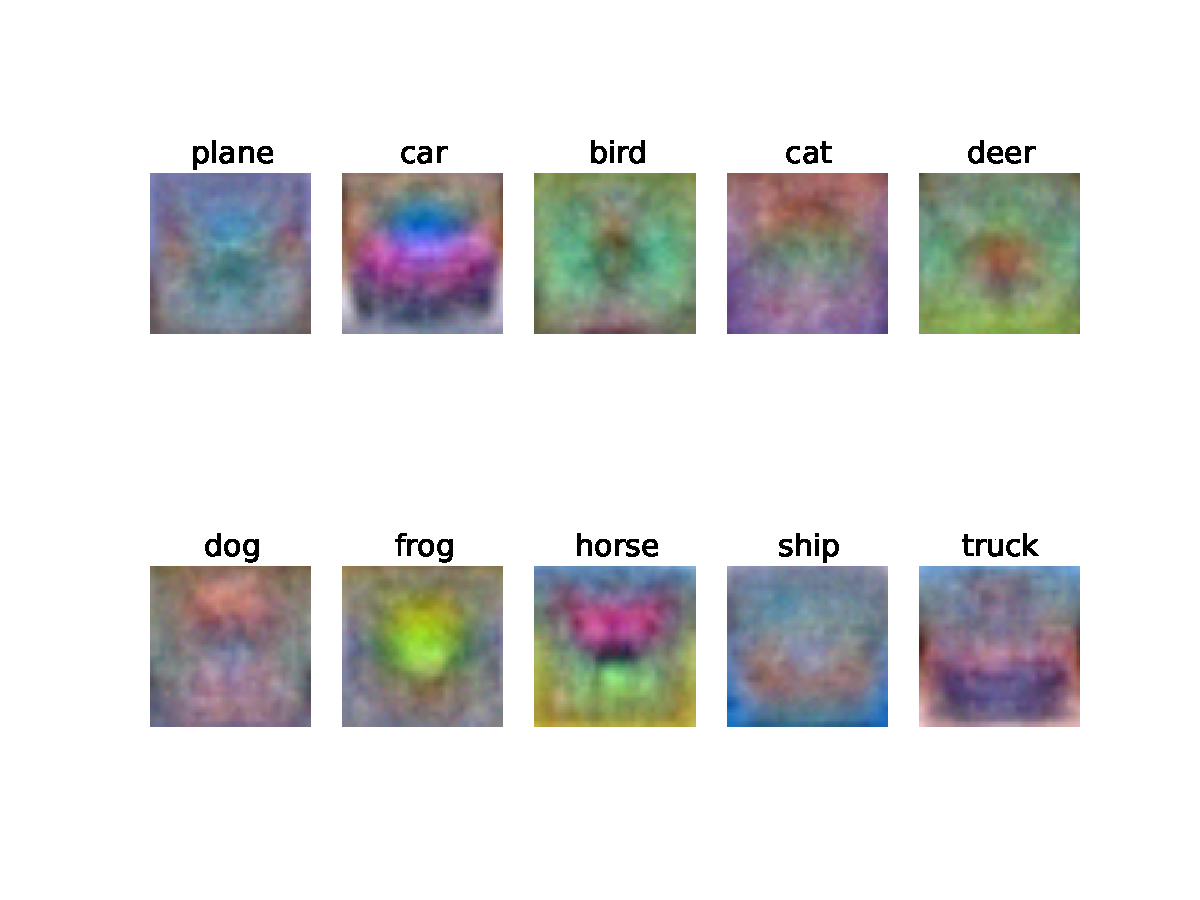
\includegraphics[width=1\linewidth]{./cifar_theta}
\caption{the visualized theta}
\label{fig:figure}
\end{figure}

\subsection{Experimenting with other hyper parameters and optimization method}
Modified the implementation for \verb|train| method of \verb|SoftmaxClassifier| class in file \verb|softmax_3_8.py|.
The \verb|train| method returns early (before max. iterations) if successive loss between iterations is less than tolerance.
A code snippet from \verb|train| method
\begin{small}
\begin{lstlisting}
      last_loss = np.mean(loss_history[-win_len:])
      loss_history.append(loss)
      curr_loss = np.mean(loss_history[-win_len:])
      if abs(last_loss - curr_loss) < tol:
        self.theta-=grad*learning_rate
        return it, loss_history
\end{lstlisting}
\end{small}
The corresponding script to evaulate batch size, learning rate, regularization parameter is in file \verb|softmax_hw_3_8.py|.
\end{document}
